%% -*- coding: utf-8-unix -*-

\chapter{課題設定}
\label{chap:problem-setting}

 \section{情報システムの構築・運用における課題}
 \label{sec:system-problem}

\ref{sec:pj-purpose}節に示したとおり、情報システムが利用者に提供するサー
ビス自体はより柔軟に変化していくことが求められるようになっている。そのた
め、サービス提供者側は、利用者に対して適切なサービス価値が提供できている
かどうかを判断していくことが求められる。

システムを構成する各要素がサービスに対する利用者要求の変化に対して柔軟に
変化していくことが求められるが、近年では特にネットワーク部分がサービス変
化の上での迅速性・拡張性の面でのボトルネックになるという状況が発生してい
る。\ref{sec:nw-test-problem}節以降でその理由と課題点について解説する。

 \section{ネットワークのテストにおける課題}
 \label{sec:nw-test-problem}

% OOD発表資料のp.2-3
% なぜ「ネットワークのテスト」を対象とするのか?
% ネットワークのテストの何が難しいのか?
% これまでネットワークのテストとしてどういったことをおこなっていたのか?

基本的な課題設定については L1patch プロジェクト試験結果レポー
ト~\cite{l1pjpoc} を参照すること。ここでは簡単に解説する。

  \subsection{なぜネットワークのテストに注目するのか}
  \label{sec:reason-to-focus-network}

\ref{sec:pj-purpose}節で示したとおり、本書では情報システムの構成要素とし
ての「ネットワーク」を対象としている。ネットワークを経由して利用可能なも
のと、ネットワークそれ自体についてではテストについての考えかたが異なる
(\figref{fig:difficulty-of-network-testing})。

\begin{wrapfigure}{r}{18zw}
 \vspace*{-3zw}
 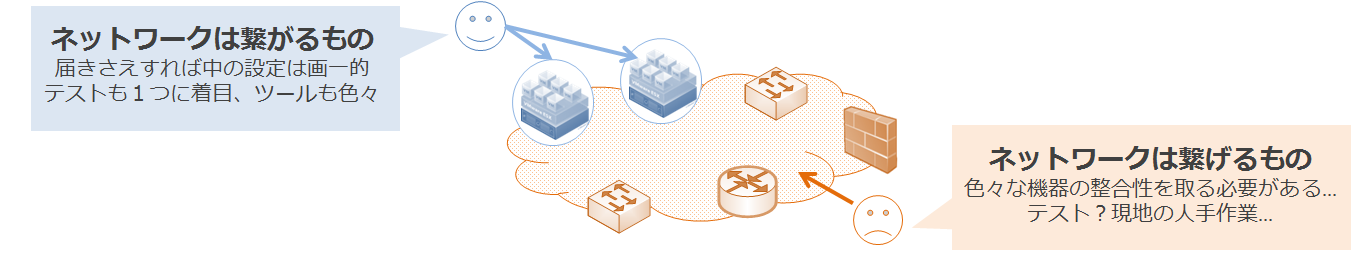
\includegraphics[scale=0.5]{img/difficulty-of-network-testing.png}
 \caption{ネットワークテストの難しさ}
 \label{fig:difficulty-of-network-testing}
\end{wrapfigure}
% \begin{figure}[h]
%  \centering
%  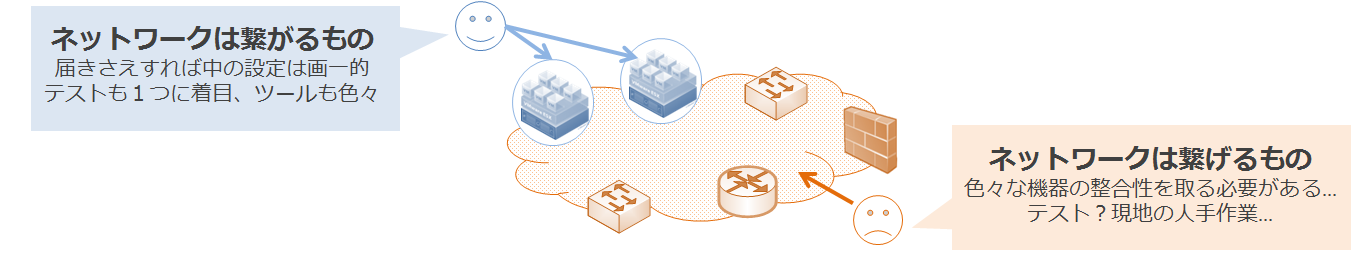
\includegraphics[scale=0.6]{img/difficulty-of-network-testing.png}
%  \caption{ネットワークテストの難しさ}
%  \label{fig:difficulty-of-network-testing}
% \end{figure}

ネットワークを経由して利用可能な機能やサービスでは、コネクティビティを前
提として作業ができるため、通信可能となっていればひとつの要素に着目して作
業可能なことが多い。しかしネットワークのテストはコネクティビティを保証す
るための作業であり、コネクティビティがあることを前提にできない。

ネットワークテスト自動化の難しさについての詳細は\ref{sec:difficulty}節で
解説するが、相互に接続される機器間の整合性の保証・テストパターンの組み合
わせ爆発・機器の物理的配置や自動操作の難しさ、といった難しさがある。こう
した理由から、ネットワークがサービス展開をすすめるうえでのボトルネックに
なる傾向がある。本プロジェクトの目的のひとつは、これらの自動化困難なもの
を可能な限り安価かつ柔軟にコントロールするための方法や実用例を提示するこ
とである。

  \subsection{自動化の難しさ}
  \label{sec:difficulty}

ネットワークで自動化がすすまない理由はいくつかあるが、ここではテストの自
動化という観点から、主要な課題について解説する。

    \paragraph{垂直統合の歴史}
歴史的に、ネットワーク機器はベンダごとに異なるOS/API(コマンド)をもち、共
通のインタフェースが存在しない。そのため、異なるベンダの機器をつかったネッ
トワークを作ろうとした場合、設定としてはおなじ操作であっても、異なる
API(コマンド)で操作する必要がある。ネットワークに対する操作の自動化はこ
れまでもおこなわれているが、機器(OS)ごと、機器の設計上の役割や運用上のオ
ペレーションごとに多数の自動化スクリプトを用意する必要があり、複雑かつ汎
用性が低い状態になっている。また、複数のデバイスを操作するうえでは、設定
が反映され動作がきりかわるタイミングなどをふまえたうえで、全体のワークフ
ローなどを考える必要があるといった課題もある。そのため自動化されるのは、
シンプルで定型的な処理にとどまることが多い。\footnote{NW機器を抽象化し統
一した方法で異なるOS/APIの機器を操作可能にする製品やOSSプロダクトなども
存在する。しかし、対応していない製品の利用にあたっては「ドライバ」とよば
れる操作対象機器のAPIや取得情報などを別途開発する必要があるなど、コスト
がかかる。APIについては、Netconf/YANGなどをベースにしたインタフェースや
データモデル標準化の動きはあるものの、現時点では実装されている機器はまだ
少数であり、ベンダ/OSごとに個別にとりあつかう必要がある、という状況であ
る。}

    \paragraph{物理的な位置の操作}
ネットワークは、情報システムの構成要素(計算機リソースなど)の物理的な配置
を抽象化する機能をもつため、ネットワークそれ自体のテストについては、物理
的な配置(場所)を考慮する必要がある。テストされていないネットワークでは、
何らかの問題によりネットワークが通信不可能になるおそれがある。リモートで
のネットワーク機器へのアクセスが不可能になってしまった場合、機器の現物を
直接操作して復旧させなければならない\footnote{こうしたリスクを回避するた
めに、リモートアクセス用のネットワークとサービス用のネットワークを物理的
に分離して設計したり(out-of-band management network)、機器コンソールをリ
モートで利用可能にするための機器(シリアルコンソールサーバ)を導入したりす
ることがある。しかし、デバイスの物理的な故障などについてはやはり何らかの
かたちで現地・現物での作業が発生する。}。こうした物理構成上の要求が発生
するテスト\footnote{例えば、リンクダウンなどの物理障害を発生させるケース、
ネットワーク機器の追加(拡張)・削除といったネットワークの物理構成(トポロ
ジ)を変更するケースなど。} は、その「実体を直接操作したい」という要求の
性質上、自動化することが難しい。

    \paragraph{テストケースの組み合わせ爆発}
ネットワークは自律分散制御され、機器相互での通信規約の整合性をとることで、
end-to-end の通信が実現される。ネットワークが狙ったとおりに動作している
かどうか、というテストでは、物理構成・論理構成を加味した多数の組み合わせ
を考慮する必要がある。ネットワークのテストパターンは、ネットワークを構成
している機能要素の組み合わせによって決まるため、構成要素の増加にともない
爆発的に増加してゆく。特に近年では仮想化技術の導入がすすみ、テストパター
ンもより多くなる傾向がある。

  \section{従来のネットワークテスト}

  % 運用の理想像や現状
  % TODO: ITHD技術交流会資料
  % \url{https://drive.google.com/drive/folders/0B2eRR_JxYJA5OFkzUFlveVlObWc}
  % p6-7 あたりとかの話をいれる

従来の「ネットワークのテスト」では、その物理構成操作の要求から、特定の場
所に人や端末を配置しながら人手でテストを実行していくという、人海戦術的な
方法がとられてきた。

しかし、ネットワーク規模や構成の大規模化・複雑化とそれによるテストパター
ン数の増大にともない、テストでパターンをすべて人手で網羅することは非常に
難しい。そのため以下のような状況(リスク)を受け入れざるをえない状況があった。
\begin{itemize}
 \item テスト作業用リソースの確保: 通常、テストをおこなうための人・機器
       の準備には制約がある。人手による作業の場合、作業コスト・時間や規
       模がどうしてもスケールさせられないため、小規模なオペレーションで
       は十分なテストができないまま本番環境での作業になる傾向がある。
 \item 一部の代表的なパターンのみをテストする: 縮小したテストケースでは
       どうしても一部の設定ミスや不整合などを見落とすリスクがある。
 \item テスト結果判断のばらつき: 手順書の解釈、操作の実行や結果の取得・
       判断などがテスト実施者に依存するため、本来問題となる事象を見落と
       してしまうリスクがある。
\end{itemize}

%%% Local Variables:
%%% mode: yatex
%%% TeX-master: main.tex
%%% End:
